\section{Phase 2}
Der in der ersten Phase erstellte Prototyp wurde dem Auftraggeber in Form eine Demo gezeigt.
Dabei sind folgenden Rückmeldungen entstanden:
\begin{itemize}
    \item Der Prototyp entspricht den Vorstellungen und erfüllt die definierten Anforderungen.
    \item Die Vorgabe, dass die Benutzerschnittstelle für Mobilgeräte ausgelegt sein soll, fällt weg.
          Sie soll nur für Desktop-Geräte ausgelegt sein.
    \item Nebst Spannungswerten soll die Applikation auch Leistungs- und THD Werte verarbeiten können.
    \item Bisher wurden sämtliche Daten künstlich erstellt.
    Diese sollen um echte Messwerte erweiter werden, welche von Auftraggeber zur Verfügung gestellt werden.
    \item Die Benutzerschnittstelle soll um die Funktion erweitert werden,
    dass eine spezifische Zeitspanne ausgewählt werden kann.



\end{itemize}

\subsection{\ac{MQTT} Datenverarbeitung}

Da neu auch die Leistungs- und THD Werte der Stromzähler verarbeitet werden sollen, wurde
die \ac{MQTT} Datenverarbeitung angepasst. Der Dataingress erwartet nun, dass nebst
den Spannungen der drei Phasen auch noch die Leistung und der THD Wert mitgeschickt wird.

Natürlich wurde auch das Datenbankschema so angepasst, dass die Daten darin abgespeichert
werden können. Zudem wurden die Tests so angepasst, dass sie auch diese Daten
mitsenden.

\begin{figure}[h]
    \centering
    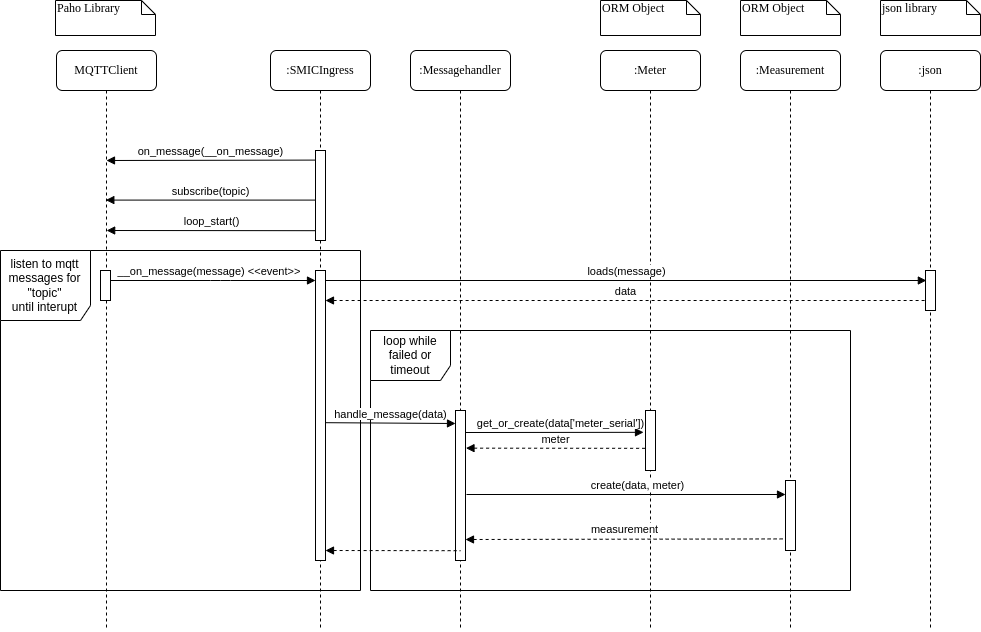
\includegraphics[width=1.0\textwidth]{gfx/dataingress-sequence}
    \caption{
        Impelemtation von Errorhandling durch den Messagehandler und einen
        retry loop.
    }
    \label{fig:dataingress-sequence}
\end{figure}

Bei der Entwicklung zeigte sich zudem, dass der Dataingress nicht sehr Stabiel
funktioniert und Sporadisch failt. Nach einiger Analyse zeigte sich, dass
die Datenbankverbindung teilweise unstabil ist. Dies aufgrund der verwendeten
SQLite Datenbank. Das Problem ist aber nicht vernachlässigbar, da auch in einer
Produktivumgebung wo beispielsweise ein PostgreSQL Server eingesetzt wird,
dieser von zeit zu zeit upgedatet werden muss.
Während dieser kurzen Zeit in der die Datenbank nicht verfügbar ist, sollten keine
Daten verlohren gehen.
Aus diesem Grund wurde wie in Abbildung \ref{fig:dataingress-sequence} aufgezeigt
ein Errorhandling implementiert. Die empfangenen Daten der Stromzähler
werden nun über einen Messagehandler abgearbeitet.
Dieser Messagehandler versucht die Daten in die Datenbank zu speichern und
reagiert im Fehlerfall.

\subsection{Fakemeter}

Um die neue Funktionalität des Dataingress testen zu können, wurde auch der
Fakemeter um Leistungs- und THD Werte erweitert.

Die Landis+Gyr stellte zudem noch einen Datensatz von echten Stromzählerdaten
zur verfügung. Damit diese echten Daten in das System eingelesen werdn können,
wurde der Fakemeter noch um einen "Batch Mode" erweitert. Das heisst
er liest das CSV File mit den Datensätzen und sendet die Daten in
gewissen Zeitabständen. Dies soll das Verhalten eines Stromzählers
möglichst realitätsnah Simulieren.

\subsection{Benutzerschnittstelle}

\subsection{Schwierigkeiten}
Schwierigkeiten während der zweiten Phase
